
%%%%%%%%% PROPOSAL -- 15 pages (including Prior NSF Support)


% From the NSF Grants Proposal Guide:
% "The Project Description should provide a clear statement of the work 
% to be undertaken and must include: objectives for the period of the proposed 
% work and expected significance; relation to longer-term goals of the PI's 
% project; and relation to the present state of knowledge in the field, 
% to work in progress by the PI under other support and to work in progress 
% elsewhere."


\required{Project Description}
\setcounter{section}{0}
\section{Introduction}
As sciences move towards more data driven research, data analysis has
become a main building block in many research disciplines.
Many advances in recent research have been driven by algorithmic improvements
in data analysis, in particular in predictive analytics and machine learning.
% [FIXME examples, cite?]
As machine learning becomes a tool for scientists across disciplines, it is
important that these analytical tools are freely available, and easy to use for
domain scientists outside of the field of machine learning.

% FIXME fast prototyping

The \sklearn{} machine learning library~\autocite{pedregosa2011scikit}, for
short \texttt{sklearn}, provides machine learning functionality
within the established --- and growing --- scientific Python
ecosystem~\autocite{benlorica, infoworld}.  \sklearn{} is an open source
library written in Python, implementing state-of-the-art machine learning
algorithm and utilities to apply these algorithms to real-world data analysis
and prediction problems.

The distinguishing features of \sklearn{} are its generic and intuitive
interface, its comprehensiveness and its
documentation~\autocite{Varoquaux_2015, benlorica}.

\emph{\textbf{Interface}} \sklearn{} provides a generic interface for machine
learning, mainly consisting of only three methods: \texttt{fit}, to build
models, \texttt{predict}, to make predictions using models, and
\texttt{transform}, to change the representation of the input
data~\autocite{buitinck2013api}.  The interface is illustrated in
Table~\ref{api} and Figure~\ref{grid_search}.  This simple and consistent
interface helps to abstract away the algorithm, and let users focus on their
particular problem. It also allows replacing an algorithm by another by
changing a single line of code. \sklearn{} utilizes the well-established NumPy library to represent data and
predictions.  NumPy is used across domains for numeric computations, and
integrating this generic representation into \sklearn{} minimizes the friction
of applying machine learning within an existing project.

\emph{\textbf{Comprehensiveness}} \sklearn{} implements a wide variety of
models for classification, regression, clustering and dimensionality reduction,
as well as methods for feature selection and feature extraction. The library
contains most of the algorithms included in standard textbooks like
\textcite{bishop2001bishop} and \textcite{friedman2001elements}, while
providing competitive implementation of state-of-the-art algorithms like
Gradient Boosting~\autocite{friedman2001greedy}, Random
Forests~\autocite{breiman2001random} and SAG~\autocite{roux2012stochastic}.  In
addition to a large selection of algorithms, \sklearn{} also contains a suite
of evaluation metrics and tools for parameter selection.

\emph{\textbf{Documentation}}
Documentation is a key ingredient to usability, and the documentation of \sklearn{}
has been widely recognized as an excellent learning
resource~\autocite{testimonials, benlorica, kdnuggetstopten, lovesklearn}. The
\sklearn{} project has strict rules on documentation and requires examples and
extensive descriptions for all algorithms.

The simple API together with the wide variety of algorithms that are
implemented in \sklearn{}, the package allows for very fast prototyping of
machine learning applications.
These key features are the ingredients leading to the wide-spread use of
\sklearn{}, and the creation of a large ecosystem of users, contributors,
maintainers and dependent packages.

\begin{table}
    \caption{Main \sklearn interface. All models have a \texttt{fit} method
    with the training data as parameter. Supervised models are also provided
    with the training targets or labels. New (usually multivariate)
    representations of the input data are produced by the \texttt{transform}
    method, while prediction of target variables (usually discrete labels or
    single continuous variables) or cluster memberships are produced with the
    \texttt{predict} method.
}
\begin{center}
    \begin{tabular}{p{.3\textwidth} p{.3\textwidth}}
    \multicolumn{2}{c}{\texttt{fit(features\_train, [labels\_train])}}\\\\
    \texttt{predict(features\_test)} & \texttt{transform(features\_test)}\\
    \cmidrule[1pt](r{1em}){1-1} \cmidrule[1pt](l){2-2}
    Classification & Preprocessing\\
    Regression & Dimensionality Reduction\\
    Clustering & Feature Selection\\
               & Feature extraction\\
\end{tabular}
\end{center}
\label{api}
\end{table}
\pagebreak

\section{Previous impact of the \sklearn{} package}
The \sklearn{} project has been widely used in academic and industrial research,
and has made its way into multiple commercial products. The
paper~\autocite{pedregosa2011scikit} describing \sklearn{} has been cited over 2750 times
according to Google scholar\footnote{We noticed that the number of citations
according to google scholar goes up at a rate of roughly 5 citations per day
during writing this proposal.}. Applications of \sklearn{} spread a multitude
of research areas, including Physics~\autocite{Baldi:2016fql, Yang:2016nnd},
Astronomy~\autocite{pereira2013spectrophotometric, bennett20141},
Biology~\autocite{misof2014phylogenomics, ritchie2014functional},
Medicine~\autocite{kamalov2015improving, ng2015computer},
Psychology~\autocite{park2015automatic,doehrmann2013predicting}, Cyber
Security~\autocite{sahs2012machine},
Oceanograpy~\autocite{sunagawa2015structure}, Social
Sciences~\autocite{driscoll2015searching, croicu2015improving} and more.

The number of 2750 is likely underestimating the use of \sklearn{} in published
research, as a search for the term ``\sklearn{}'' yields 4850 results.
Other ways to measure the use and impact of \sklearn{} is the engagement with
the project via code contributions, downloads, support requests and other
community interactions.
According to the email addresses used for code contributions (a conservative
estimate), 40 researchers and students from at least 23 US universities
\emph{contributed code} to \sklearn{}, indicating wide-spread academic use.
These institutes include University of California Berkeley, Brown University,
Carnegie Mellon University, Columbia University, Duke University, Harvard
University, Massachusetts Institute of Technology, New York University,
Stanford University, and University of Washington.
The total number of unique contributors to the project is about 700.
%
The \sklearn{} mailing list has 1666 subscribers, including 70 email
addresses from ``edu'' domains, across 43 institutes.
%
On the question-answering site Stack Overflow, there are around 4500 questions
tagged as \sklearn{} related, with 222 questions asked within the last 30
days of this writing.

For the last 5 years, the scientific Python conference SciPy has had a \sklearn{} tutorial,
showing the great demand for education in using machine learning and \sklearn{} in particular.
In 2015, the tutorial was so overbooked that a second session was held.

\sklearn{} has become the center of the machine learning ecosystem in the scientific Python community,
with several domain-specific packages relying on and extending its functionality.
Prominent examples of scientific software packages depending on \sklearn{}
for machine learning include \texttt{astroML}~\autocite{van2013openml} for astronomical
data, \texttt{nilearn}~\autocite{abraham2014machine} for neuroimaging, \texttt{MNE-Python} for MEG
and EEG data, \texttt{librosa}~\autocite{mcfee2015librosa} for audio and musical data,
\texttt{nltk}~\autocite{bird2006nltk} and \texttt{rosetta} for Natural language processing, \texttt{bcbio} for
RNA sequence analysis, \texttt{scikit-allel} for genetic variation data, and \texttt{rootpy} for
integration with the \texttt{ROOT} scientific software framework.
The main use of \sklearn{} is outside of these major open source packages, though,
as stand alone library for data analysis. Using the GitHub repository, we found
about 40.000 Jupyter notebooks---a format for interactive computing with
Python---that use \sklearn{} at the time of writing.

\begin{figure}
    \begin{center}
    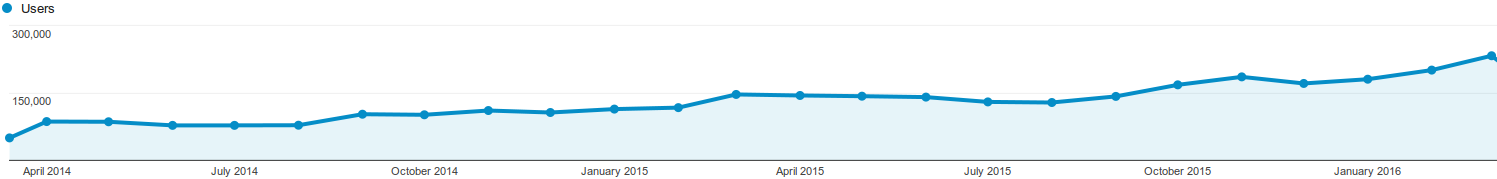
\includegraphics[width=.95\linewidth]{scikit-learn_site_visits}
    \end{center}
    \caption{Evolution of monthly Scikit-learn website views (unique visitors).}
    \label{traffic}
\end{figure}

The \sklearn{} website containing the documentation was visited by over
230.000 users in March 2016, upward from 200.000 users in February and 180.000
users in January, reflecting the growth of the \sklearn{} user community. See
Figure~\ref{traffic} for a long-term trend.

\sklearn{} has become so popular in teaching and data science applications that
several books have been written about the use of
\sklearn{}~\autocite{garreta2013learning, hackeling2014mastering,
hauck2014scikit, raschka2015python}. Another book, titled ``Introduction to
machine learning with Python'' is currently in preparation by PI M\"uller.

\section{Proposed Work}
Despite the extensive documentation, applying machine learning using \sklearn{}
still requires expert knowledge about:
\begin{itemize}
    \item What kind of models to use for a given task.
    \item What kind of feature extraction and preprocessing is required for a model.
    \item What parameters to tune, and in which ranges.
\end{itemize}

While it is easy for a scientist to create a working model, this model might not
be optimum, and they could obtain a much better model using more expert knowledge
in machine learning to answer the questions listed above.
However, the need for this expert knowledge can be eliminated at least partially
using recent developments in model selection and meta-learning.

Funding form this proposal would enable a concentrated effort to include more
automatic model selection in \sklearn{}, and therefore lower the barrier to
entry for applying machine learning even further.
The components of the proposed work are:
\begin{itemize}
    \item Improving the existing pipelining facilities for more automatic feature extraction.
    \item Recommend explicit sets of parameters to tune for each algorithm,
        together with recommended ranges, based on large-scale experiments.
    \item Integrate methods for Bayesian optimization for parameter selection.
    \item Integrate meta-learning for automatic model selection.
\end{itemize}
Together, these additions to the \sklearn{} ecosystem will enable more widespread use,
in particular by scientists outside of the field of machine learning, and improve results
of existing users.

\section{Intellectual Merit}
Improving automation in model selection and preprocessing in \sklearn{} will have far-reaching
implications for existing and future applications of machine learning.
Research projects that already use \sklearn{} for machine learning will be able to adapt better
models with minimal changes to their workflow, potentially improving their research outcomes.
For research projects that are not relying on machine learning yet, including a model
from \sklearn{} will be much easier and require much less expert knowledge.

Developing more automated model selection requires extensive benchmarking and evaluation
on a diverse array of machine learning problems. Such a large scale evaluation,
in the spirit of \textcite{caruana2008empirical, caruana2006empirical} and more
recently \textcite{feurer-nips2015} can provide important insights into the state
of the art in machine learning. This proposal will not only provide results of
extensive evaluation, it will also result in improved infrastructure
for large scale studies of algorithms.

\section{The \sklearn{} package and ecosystem}
The \sklearn{} machine learning library is an open source library for the
Python programming language, distributed under a BSD license.
It is developed largely by a community of volunteers, with some support from
INRIA, Telecom ParisTech, Paris-Saclay Center for Data Science and through PI
M\"uller as part of the Moore-Sloan Data Science Environment at NYU\@.
The package was first released in 2010, and new releases are made semi-annually.
The development team has 38 members, and releases and project management are
coordinated between PI M\"uller and Olivier Grisel at INRIA\@.
There have been approximately 670 contributors to the project so far, demonstrating
the wide community engagement, with each release typically including changes
from 100 to 150 contributors.

\subsection{Project Description}
The \sklearn{} project focusses on efficient and easy-to-use implementation
of state-of-the-art machine learning algorithms that are useful for a wide
audience of machine learning practitioners in research and commercial
applications~\cite{pedregosa2011scikit, buitinck2013api}.
Implemented algorithms include Support Vector Machines, Random Forests, Gradient Boosting,
Non-Negative Matrix factorization, Independent Component Analysis, K-Means, DBSCAN, Isomap,
t-SNE and many others. To facilitate easy evaluation and model selection, \sklearn{}
implements metrics like the $R^2$, AUC, Adjusted Rand score, Mutual information, Average precision
and many more. Additionally, a framework for cross-validation and parameter selection is
provided, allowing parameter tuning with very little effort.

Given that \sklearn{} is mostly developed and maintained by volunteers,
one of the core principles of \sklearn{} is to lower the barrier for new developers,
and keep the complexity of the code as low as possible, to simplify maintenance.
The success of this approach can be seen in the large number of contributors to
the project.

\subsection{Interface and extensibility}
The simple interface of \sklearn{} has received substantial recognition for its user friendly design.
The main functionality of machine learning models can
be summarized using just three functions (see Table~\ref{api}):
\begin{labeling}{\texttt{transform}}
    \item[\texttt{fit}] for building models
    \item[\texttt{predict}] for creating predictions
    \item[\texttt{transform}] for generating new representations.
\end{labeling}
Creating a custom model or preprocessing method using this interface is very simple,
and a way in which many users extend the functionality. The \sklearn{} documentation
has comprehensive documentation on the conventions and interfaces in \sklearn{},
to promote the creation of custom extensions.
The \sklearn{} library even has a generic test framework that allows users to
test their own implementation against the behavior expected by \sklearn{}.

\subsection{Impacts in research}
\sklearn{} has had an impact first in the field of machine learning,
where it continues to provide a baseline for comparison, as well as a
framework in which to develop and evaluate new methods.
The much broader omni-disciplinary impact is in providing easy-to-use
tools for solving machine learning tasks. By providing a collection
of methods with a simple and consistent interface, researchers
can easily explore different solutions to their machine learning problems,
with a large collection of well-tested and well-established algorithms
at their finger tips.
The adoption of \sklearn{} in research can be seen in the large number
of citations (over 2750 according to Google scholar) as well as in the development
of more domain specific solutions build on \sklearn{}.
According to the email addresses used for contributions, researchers and students
from at least 23 US universities \emph{contributed} to \sklearn{}, indicating wide-spread use.

\subsection{Impacts in education}
In addition to being widely used as a toolkit by practitioners,
\sklearn{} is also popular in teaching machine learning.
The emphasis on accessibility, usability and documentation within
the \sklearn{} project makes it ideal for an introductory
course in machine learning, and allows access to a wide variety
of algorithms. \sklearn{} is particularly popular in teaching
Data Science courses that focus on making inferences about
a particular data set, rather than the mathematics that go into
particular ways to solve machine learning problems.
Data Science courses are usually targeted at a broad spectrum
of students with mixed backgrounds, providing them
with the data analysis tools useful across domains.

Academic teaching has made use of \sklearn{} at institutes including New York
University, Brown University, Duke University, University of California
Berkeley, Stanford University, Princeton University, Columbia University,
University of Pennsylvania, Georgetown University, Cornell University and
others.

\subsection{Reproducibility, democratization and openness}
An important contribution of \sklearn{} has been in providing a common
ground for scientists to base their research on. Reimplementing
and algorithm from a text book or the description in a paper is often not
straight-forward, and slight differences in implementation details can
lead to different experimental outcomes. By providing shared, open and 
accessible infrastructure that is used by many research groups,
\sklearn{} facilitates reproducibility of algorithmic results.
The open source nature of \sklearn{} means that everybody can have access
to advanced machine learning within the scientific Python ecosystem,
without having to spend money on commercial analysis software like Matlab,
SPSS or Stata.

\subsection{Integration in scientific Python ecosystem}
\sklearn{} is firmly rooted in the scientific Python ecosystem, and has been
one of the catalysts of its success~\autocite{benlorica, infoworld}. \sklearn{}
builds heavily on the foundations on \texttt{NumPy} and \texttt{SciPy}, and
integrates easily with the popular pandas library for data analysis and the
\texttt{matplotlib} library for plotting and visualization.
\sklearn{} has been included in several scientific Python distributions, such
as the popular cross-platform ContinuumIO Anaconda and Enthought Canopy
distributions, as well as the Python-xy distribution for Microsoft Windows.

The succinct interface of \sklearn{} also lends itself well to interactive
data exploration and model building within the Jupyter Notebook environment.
As mentioned previously, searching for Jupyter notebooks containing
\sklearn{} code on the GitHub code hosting platform yields about 40000
results.

\begin{figure}
    \begin{minted}{python}
    # model fitting and prediction with fixed parameters:
    from sklearn.ensembled import RandomForestClassifier
    forest  = RandomForestClassifier(max_depth=10, max_features=3)
    forest.fit(features_train, labels_train)
    forest.predict(features_test)

    # model fitting and prediction with grid-searched parameters
    from sklearn.model_selection import GridSearchCV
    parameter_grid = {'max_depth': [1, 3, 10], 'max_features': [1, 2, 3]}
    forest_grid = GridSearchCV(RandomForestClassifier(), parameter_grid)
    forest_grid.fit(features_train, labels_train)
    forest_grid.predict(features_test)
    \end{minted}
    \vspace{-5mm}
    \label{gridsearch}
    \caption{Current interface to scikit-learn classification and parameter
        selection. The user needs to select parameters of importance (here
        \texttt{max\_depth} and \texttt{max\_features}), and values for these
        parameters to test (here 1, 3, 10 for \texttt{max\_depth} and 1, 2, 3
        for \texttt{max\_features}).}
\end{figure}

\section{Proposed Enhancements}
While the \sklearn{} package is under constant development by a large community
of volunteers, the size and widespread adoption of the package result in much of this
time being spend on maintenance and usability improvement, leaving little room
for larger scale efforts to include major changes. The goal of this proposal
is to implement major usability and automation features in \sklearn{}, decreasing
the domain expertise required to successfully implement machine learning models.
We propose to improve three aspects of applying machine learning models that
currently require substantial expert knowledge: parameter selection, model
selection and data preprocessing.

\subsection{Default Parameter Ranges}
Nearly all machine learning models come with parameters to set or tune
to achieve good predictive performance. The most wide-spread way to adjust
these parameters is grid-search with nested cross-validation.
Grid-search consists of an exhaustive search over all possible combinations
of the parameters under consideration. Example code for the process is given
in Figure~\ref{gridsearch}.
A major hurdle in applying grid-search in practice is that algorithms
often have many different tuning parameters, making exhaustive search
over all of them infeasible. However, in practice only a small subset
of the parameters is usually critical for good performance. This set,
and good candidate values to try, are often not well-documented in research and
not included in text books.
The \sklearn{} documentation tries to give guidelines, but these can be hard
to find and understand by people outside of machine learning.
We propose the inclusion of a programmatic way to query for the parameters
to adjust for each model, and what good parameter ranges are.

While there is some community consensus on this issue, we want to back
up our choices by large scale experiments on existing benchmark libraries
of datasets, like OpenML~\autocite{van2013openml}.
\begin{labeling}{Task 1}
    \item [Task 1] Benchmark parameter ranges of commonly used supervised models.
    \item [Task 2] Provide default parameter ranges inside \sklearn{}.
\end{labeling}

\subsection{Bayesian Optimization Based Parameter Selection}
An alternative to exhaustive grid-search in selecting parameters is using
Bayesian optimization to iteratively improve the tuning parameters of a
model~\autocite{NIPS2011_4443, shahriari2016taking, NIPS2012_4522}.  This
technique has been well-established in the machine learning literature, and
there are several implementations available.~\autocite{bergstra2013hyperopt,
feurer-nips2015, komer2014hyperopt, snoek2015scalable}.  However, these
algorithms have not made its way into the software used by domain scientists
that use machine machine learning algorithms as tools in their research.
By incorporating a robust and efficient implementation into \sklearn{},
this proposal will bring the benefits of the recent advantages in model selection
from the machine learning community to the scientific users of \sklearn{}.
\begin{labeling}{Task 3}
    \item [Task 3] Benchmark and integrate Gaussian Process based parameter optimization.
    \item [Task 4] Benchmark Random Forest based parameter optimization.
    \item [Task 5] Integrate \texttt{auto-sklearn} Bayesian optimization with \sklearn{}.
\end{labeling}

\subsection{Automatic Preprocessing Selection}
\sklearn{} has a build-in mechanism to construct ``pipelines'' which are complex 
machine learning workflows, consisting of operations like feature extraction,
feature transformation, feature selection and predictive models.
All evaluation and parameter selection mechanisms in \sklearn{} can operate
on these pipelines.
However, selecting which steps to chain together, that is which preprocessing
to use for which model, is left to the user. Currently there is no
automatic process to compare different pipeline constructions, even though
the right combination of methods is often crucial but not obvious in practice.
We propose to extend the model selection and pipelining framework in \sklearn{}
to allow automatic selection of pipeline steps.
To facilitate automatic preprocessing selection, we will also programatically
define input and output conditions of different processing steps, such
as requirements for sparse data, dense data, non-negativity of features and others.
\begin{labeling}{Task 9}
    \item [Task 6] Allow setting of pipeline steps in \sklearn{} parameter searches.
    \item [Task 7] Implement tagging of pre-conditions and post-conditions for data transformations.
    \item [Task 8] Refactor \sklearn{} testing to validate pre-condition and post-condition tags.
    \item [Task 9] Collect common encoding schemes for categorical and
        continuous data in a \sklearn{} compatible way.
\end{labeling}

\begin{figure}
    \begin{center}
    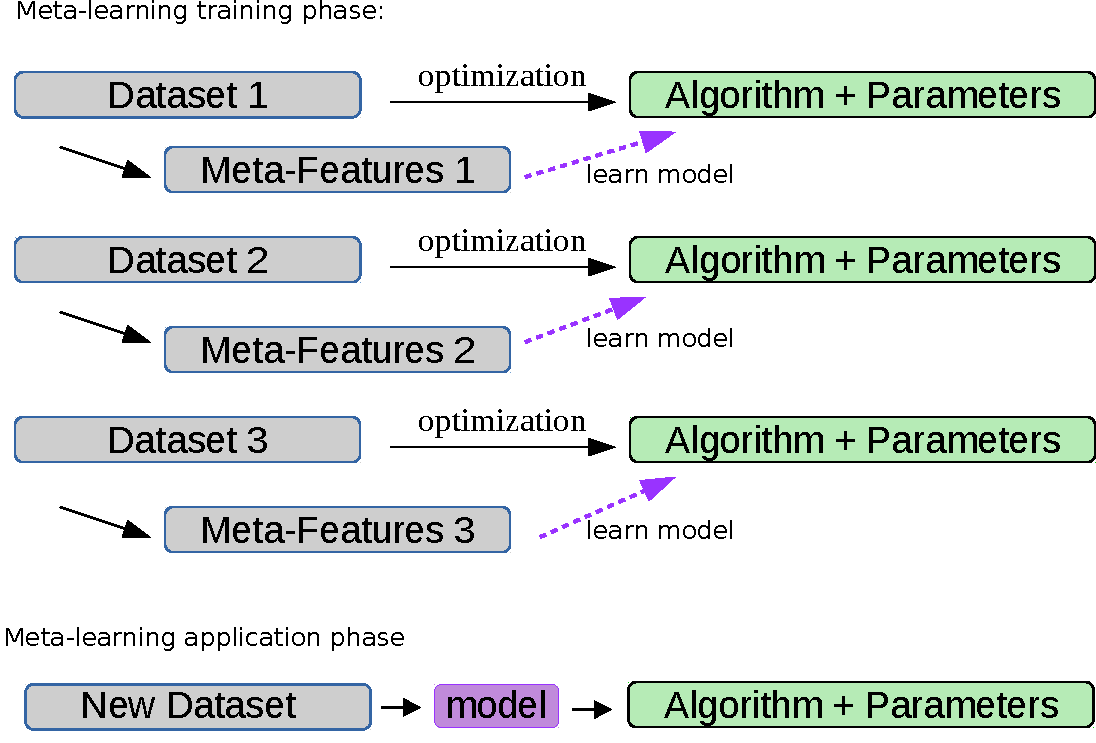
\includegraphics[width=.6\linewidth]{meta-learning-diagram.pdf}
    \end{center}
    \caption{Illustration of meta-learning. First, good parameter values for
        each training dataset are found using optimization. Each dataset is
        then represented via meta-features. A Machine learning model is learned
        to predict parameter settings from the meta-features. For a new
        dataset, the machine learning model can be used to find good
    parameters, removing the costly optimization step.}
    \label{meta-learning}
\end{figure}

\subsection{Meta-Learning}
Going beyond brute-force search or even Bayesian optimization for parameter and
model selection, it is possible to use machine learning to recommend suitable
algorithms and parameters based on properties of a data set, such as number of
samples, number of features, number of classes and statistical properties of
the features~\autocite{luo2015review, feurer-nips2015}.
Given these meta-features and the best pipeline and parameters found using
Bayesian optimization or grid-search, it is then possible to build a machine
learning model to predict what the best classifier for a new dataset would be.
This prediction based on meta-features is computationally much less demanding
than searching for a model and parameters from scratch for each new dataset. The process
is illustrated in Figure~\ref{meta-learning}
Meta-learning allows the principled incorporation of expert knowledge as encoded
in the collection of datasets used for training.
While there are working implementations of meta-learning available
(\texttt{autoweka}, \texttt{auto-sklearn}),
these projects are currently in a ``research software'' state. Making these methods
available to the wider scientific audience will require substantial engineering
efforts. The above steps of incorporating Bayesian optimization and automatic
preprocessing selection will lay the foundation to enable meta-learning within the
\sklearn{} framework.
\begin{labeling}{Task 10}
    \item [Task 10] Refactor \texttt{auto-sklearn} to make use of new pipeline and transformation conditions.
    \item [Task 11] Benchmark meta-learning features on OpenML datasets.
    \item [Task 12] Create meta-learning package from the previously build
        components, with full user documentation and test coverage that is
        installable via the Python package manager.
\end{labeling}

\section{Enabled Research Opportunities}
The proposed project will benefit researchers inside the machine learning field,
but more importantly will have an impact on new and existing applications of machine
learning across many domains of science.

\subsection{Reduce Barrier to Entry}
One of the premier goals of this project is to lower the barrier to entry
to applying machine learning in scientific applications even further.
\sklearn{} with its intuitive interface and comprehensive documentation
has made machine learning algorithms available to a much wider audience.
However, selecting and tuning models still requires machine learning expertise.
The wealth of algorithmic choices for solving a particular research problem can be
overwhelming to researchers from other disciplines. By building more automated
abstractions on top of the existing machine learning algorithms in \sklearn{},
we will enable researchers to apply powerful models without learning
the characteristics and particularities of specific methods.
This will ease the adaption of machine learning for many researchers
that have not yet made use of machine learning.

\subsection{Improved Rapid Prototyping}
In data science, exploration is often limited by the human interactions needed to analyze data.
Being able to rapidly ask many research questions about a dataset or task of interest allows
quick exploration of hypotheses and speeds up research.
Data preprocessing and model tuning is often a laborious and time-consuming part of analysis.
More automation in applying machine learning means that a researcher can ask a scientific
question in terms of a machine learning problem, start the automated machinery to
search for a model, and then continue exploring the data, without having to closely monitor
the process on the model. 
This frees up research time to investigate other questions, instead of trying to
find the right model to answer the first.

\subsection{Plug-In Replacements}
Many researchers are already using \sklearn{} models in their projects, as witnessed
by the citations and other usage statistics we reported above. As the automation features
in this project will provide the same interface as the existing models, researchers
can simply replace the models in their existing projects by an automatic model search.
This will lead to better predictive results by simply changing two lines of code.

\subsection{Large-Scale comparisons}
Lastly, by providing a reproducible and open large-scale comparison of machine learning
methods on a wide variety of datasets, we provide guidance for future research
in machine learning itself.
In the tradition of \textcite{caruana2006empirical} and
\textcite{caruana2008empirical}, we will identify strengths and weaknesses of
existing models, to allow dissemination by the wider machine learning
community.

\section{Community Engagement, Outreach, and Sustainability}
\subsection{Community integration}
As co-maintainer part of the core team of developers of \sklearn{}, PI
M\"uller is well integrated into the development process of \sklearn{}.
This will enable the direct incorporation of many of the proposed enhancements
into the \sklearn{} main package.
It will also provide a wide exposure of the proposed activities to the
\sklearn{} community. We anticipate contributions to the proposed
project from the open source community from day 1 of this project.
The close connection of PI M\"uller to the \sklearn{} user community will
also enable us to closely interact with users to ensure covering common use cases,
instead of creating software solutions in the vacuum.

\subsection{Software Quality and Testing}
The \sklearn{} project has a history of high standards on code quality, reviews and testing.
Each new contribution to \sklearn{} needs to be reviewed by at least two senior team members
in addition to the contributor. Often, many more reviews are performed. The
pull-requests (contributions) made to the project have on average 16 comments
made by developers and maintainers on improving code quality and algorithms.

\sklearn{} has an extensive testing suite, covering 94\% of lines of code in the project.
The test suite consists of unit tests, integration tests and algorithmic tests.
There is automated testing performed on all algorithms in \sklearn{} that ensures a common
interface and user experience.
All tests are run as continuous integration tests on Microsoft Windows and Linux, and using
multiple versions of Python as well as multiple versions of \texttt{NumPy} and \texttt{SciPy}, ensuring
compatibility with a wide array of end-user systems.

In adding to the \sklearn{} project, this proposal will leverage the existing infrastructure
and quality standards inside the \sklearn{} community, ensuring high quality, well-tested code.

\subsection{Documentation and Distribution}
Similar to the processes for reviews and testing, the proposed project will
also be able to leverage the well-tested documentation and distribution
infrastructure of \sklearn{}.
As mentioned above, there is continuous integration testing on multiple operating systems,
ensuring compatibility and seamless installation across platforms.
The integration services are also set up to build binary releases of the \sklearn{} package
for distribution, so that making a release that can be installed on any platform is as
easy as tagging a commit as a release.
The continuous integration servers are also set up to rebuild the documentation on a per-change
basis, so that the documentation website (for the development version) is always up-to-date
with the current code.
\sklearn{} has a history of increasingly high standards for documentation,
requiring a description of algorithms, use cases, important parameters and theory,
as well as compelling examples~\autocite{lovesklearn, benlorica}. This culture of comprehensive and accessible documentation
will carry over to any additions made as part of this proposal.

\subsection{Sustainability Plan}
The \sklearn{} community has grown substantially over the years, and volunteer efforts
are by far the largest component of work contributed to the project.
When people do leave for personal reasons, often time commitments made as part
of more senior academic positions, the project has managed to smoothly integrate new
contributors into the core team. Due to substantial efforts to ease the barrier
of entry for contributors, the \sklearn{} team is able to attract new volunteer
core developers on a regular basis, and has successfully transitioned from one
``generation'' to the next multiple times. 

While there is an active community around \sklearn{}, it is very hard to make
major changes based on volunteer efforts alone. New models that are added have
often been the product of internships or the Google Summer of Code program.  We
therefore propose to hire a full time developer as part of this proposal to
greatly accelerate the progress in terms of usability and automation. Once
the proposed features are included into the project, maintaining them will be
possible using the resources provided by the community. 
% FIXME this argument needs to be way better.

% GSOC somewhere? Broader impacts?
\subsection{Diversified Outreach}
As part of this proposal, we plan to hold an annual workshop or coding sprint
in the New York area to engage scientists, and introduce them to contributing
to open source. Past experience has shown that many people are interested
in contributing to open source, but are often intimidated by the process.
By hosting an open and interactive workshop, we aim to broaden the base
of contributors to the \sklearn{} project.
Unfortunately open source projects often lack diversity in their core team,
and most core contributors of scientific Python packages being men.
We hope to improve the situation by partnering with local and national
organizations for women in machine learning and women in the Python community,
to engage more female developers.
We plan a weekend-long workshop, which will give a short introduction to
contributing to open source, followed by two days of hands-on contributions to
\sklearn{}.
From prior experience~\autocite{meetupsprintSF}, it is possible for new
contributors to make meaningful changes within one or two days, so that
attendants will go home with a contribution in the project. After pioneering
this model with \sklearn{}, our goal it to engage with other open source
projects with core developers local to New York (\texttt{pandas},
\texttt{matplotlib}) to increase the impact of the workshop.

\section{Project Coordination and Evaluation Plan}
\subsection{Project Coordination and Timeline}
PI M\"uller is a core developer and co-maintainer of \sklearn{} and deeply integrated
into the community around it. The PI will lead the execution of the project and the integration
into \sklearn{} and the \sklearn{} ecosystem.
The developer will implement the new features and review changes proposed by
the \sklearn{} community. The developer will also perform large-scale
benchmarking experiments to validate the effectiveness of the parameter
recommendations and the automation features.  The PI and developer will both
interact with the greater community via issue trackers, mailing lists and
chat rooms. The developer and PI will share working space to facilitate
collaboration. The timeline of the project is illustrated in Figure~\ref{timeline}

\begin{figure}
    \begin{ganttchart}[
    hgrid,
    x unit=0.28cm,
    y unit chart=.5cm,
    compress calendar,
    time slot format=isodate-yearmonth,
    bar/.append style={fill=blue!50},
    include title in canvas=false,
    bar top shift=0.2,
    bar height=.6,
    bar label node/.append style={align=left, text width=6cm},
    y unit title=.3cm
    ]{2016-11}{2019-10}
    \gantttitlecalendar[title/.style={draw=none, fill=none}]{year}\\
    \gantttitlecalendar[title/.append style={fill=black!10}, title label font=\tiny\color{black!10}]{year}\\
    \ganttbar{1 Benchmark parameter ranges}{2016-11}{2017-04} \\
    \ganttbar{2 Provide default ranges}{2017-05}{2018-4} \\
    \ganttbar{3 GP-base BO}{2016-11}{2017-10} \\
    \ganttbar{4 RF-based BO}{2017-05}{2017-10} \\
    \ganttbar{5 Integrate with \texttt{auto-sklearn} BO}{2017-11}{2018-10} \\
    \ganttbar{6 Searching pipeline steps}{2016-11}{2017-04} \\
    \ganttbar{7 Transformation conditions}{2016-11}{2017-04} \\
    \ganttbar{8 Integrate conditions in sklearn}{2017-05}{2017-10} \\
    \ganttbar{9 Feature encodings in sklearn}{2017-11}{2018-10} \\
    \ganttbar{10 sklearn $\leftrightarrow$ \texttt{auto-sklearn} sync}{2017-11}{2018-10} \\
    \ganttbar{11 Benchmark meta-learning}{2017-05}{2018-04} \\
    \ganttbar{12 Meta-learning packaging}{2018-11}{2019-10}
    %\ganttlinkedbar{Task 2}{3}{7} \ganttnewline
    %\ganttbar{Final Task}{8}{12}
    \end{ganttchart}
    \caption{Project timeline}%
\label{timeline}
\end{figure}

\subsection{Need for a Senior Developer}
As many of the contributors of \sklearn{} work in academic environments,
often the time they have available to do volunteer work on open source is
inversely proportional to their seniority.
Consequently, there are many junior contributors with good coding skills,
but less developed project management and timing skills.
Therefore it is paramount to have a senior developer to lead the efforts
on major new features, to ensure roadmap and scoping are useful and realistic.
\sklearn{} currently has around 430 open contributions (GitHub pull requests)
that require code review and oversight from a senior developer to be integrated
into the project. This exemplifies the size of the community of contributors,
but also points out the bottle neck in terms of senior developers that
have enough machine learning and software development expertise to judge
the usefulness, efficiency and correctness of the proposed additions.


\subsection{Evaluation}
The success of an open source project is notoriously hard to measure. The
success and impact of an addition to an existing open source project even more
so. Open source software has many paths of distribution; in case of \sklearn{},
these are the Python package manager (pypi), pre-packaged distributions like
anaconda, canopy and Python-xy, the package managers of Linux distributions (like dpkg and rpm)
and downloads directly from the GitHub repository. Most of these distributions paths are hard
or impossible to track. The Python package manger for example reports over 500.000 downloads of the last
release, which is likely to be inflated when taken as a measure of users.
On the other hand, the number of citations of the relevant
pape~\autocite{pedregosa2011scikit}, over 2750, is likely to be much lower than
the number of papers actually using the \sklearn{} library in their research.

To get a more comprehensive picture of the adoption of an open source software
package, we can look at the citation and download counts together with other
statistics, like the number of discussions on the question answering site
Stack Overflow, the number of contributors, the number of people writing to the
mailing list, the number of projects depending on the package etc.  These
numbers are particularly meaningful when compared to other projects with a
similar scope.

We will develop the more novel features outside of the \sklearn{} package, which will
facilitate measuring the impact of the proposed additions. The impact of contributions
to the \sklearn{} package, however, is harder to measure. One simple measure of impact
is that some the proposed features will actually be integrated into \sklearn{}.
Even though the PI is tied into the core developer team, there is no guarantee
a contribution will be accepted unless it meets the very high standars
on code quality, usability and usefulness set by the community.

Another direct measure of impact is to count use of a particular function in
code available on GitHub. As more and more research groups use version
control fore their experimental code, and publish it as open source, a growing
number of groups and individual researchers have a presence on GitHub.com.
Counting the use of the added functionality, in particular inside Jupyter
Notebooks, provides great insight into the use of the proposed additions in
research and data analysis.


\section{Collaborations}
\subsection{Diversity in open source in collaboration with WiMLDS}
While the \sklearn{} community is quite successful in finding new contributors,
unfortunately only one of the 38 \sklearn{} core developers is a woman.
Similar issues can be found in related packages, with \texttt{NumPy} having no
women among the 13 core developers and \texttt{SciPy} having one women out of
22 core developers.

To increase diversity, this proposal includes an annual workshop to increase
contributions to the open source community, in particular targeted at women.
To this end, we collaborate with the ``Women in Machine Learning and Data Science''
meetup group located in New York, a community of over 1500 (mostly) female data science and
machine learning experts.

\subsection{Collaboration with \texttt{auto-sklearn}}
The \texttt{auto-sklearn} project~\autocite{feurer-nips2015} currently provides
a research prototype of meta-learning with Bayesian optimization for parameter
selection. One of the main goals of this proposal is to transfer the research
within the \texttt{auto-sklearn} project to a easy-to-use and well-documented
library, integrated within the \sklearn{} ecosystem. To this end, we will
collaborate with the \texttt{auto-sklearn} team, building upon their insights
and technologies. Frank Hutter committed to providing the support of his group
to integrate our additions to \sklearn{}, such as the default parameter ranges
and automated preprocessing selection into their software, while in turn
providing the necessary domain knowledge to reproduce their research results in
a user-friendly library.

\subsection{Collaboration with OpenML}
Evaluation and benchmarking on real-world datasets are essential to this
proposal, in providing guidance for good parameter ranges, and assessing the
success of automatic model selection methods. The OpenML
project~\autocite{van2013openml} provides a quickly growing database of machine
learning datasets with associated tasks, including classification and
regression~\autocite{vanschoren2014openml}. At the time of this writing, there
were nearly 20.000 datasets hosted on OpenML, ranging from classical datasets
like MNIST and small toy datasets like the iris and wine datasets, to large
scale datasets with millions or even tens of millions of samples, ranging from
biological, medical and physical datasets to commercial applications. This
growing collection or research datasets provides the basis of our assessments,
and ensure relevance of our effort across research domains.  Joaquin Candela
committed to improving and maintaining the Python interface for the OpenML
platform, and improving the support for \sklearn{} based models.

\subsection{Early Adopters}
The following researchers have committed to being \emph{early adopters} of our
software products. They will use the improvements and packages in their
research projects, and provide valuable feedback for ensuring usefulness of the
software for a variety of research applications:

\begin{labeling}{\textbf{Experimental Particle Physics}}
    \item[\textbf{Experimental Particle Physics}] Prof. Kyle Cranmer (NYU) committed to have his group be an early
    adopter of the proposed project for their work on searching new phenomena at the Large Hardron Collider.
    \item[\textbf{Astronomy}] Prof. David Hogg (NYU) commited to have his group be an
        early adopter of the proposed project for his work on analyizing
        telescope imaging data for extracting astronomical principles.
\end{labeling}

\section{Broader Impacts of the Proposed Work}
The proposed project has a wide-reaching impact on the practical use of
machine learning in research, and on how machine learning can be taught to
 scientists from other domains.
Providing more automatic model selection will drastically lower the barrier
to entry to using machine learning for people without domain expertise
in machine learning.
Additionally, it will save time and effort spend by researchers doing
model selection by hand, replacing their effort by an automated process.
This will make researchers more productive, and will allow them to focus
on their area of study.

Automation, coupled with publishing the results of large scale experiments will
also provide help in education. Currently, often parameters and preprocessing
are seen as undocumented expert knowledge, derived from personal experience.
Formalizing this knowledge, and providing a database of experiments, will allow
students to quickly master the necessary steps to apply machine learning in
practice.

The proposed project will also enable us to grow the open source community
within the data science and machine learning community.  In particular, the
position of \sklearn{} as a popular and valued research library enables us to
reach out to a broad community of users.  The prominent status of \sklearn{}
enables us to influence the current make-up and values of the scientific open
source ecosystem.  We proposed to host ``coding sprints'' to introduce
outsiders to contributing to open source and enlarging the number of
contributors even further. This event will be held collaboration with the New
York based Women in Machine Learning and Data Science group, to grow the number
of female contributors in particular. 

% as in the project summary, broader impacts must be called out separately 
% in the project description.  You may be able to give more specific
% examples, or discuss how you've previously achieved these impacts.
% It should be similar, but not identical, to the Broader Impacts statement
% in the project summary

\section{Results From Prior NSF Support}
Dr.\ Andreas M\"uller has not been a PI or co-PI on an NSF grant.
